\chapter{Theory}


\section{Standard Model}
    
    The Standard Model of particle physics has proven excellent at describing particle interactions up to the energy scale of modern colliders (~ TeV) and with the discovery of a Standard Model like Higgs Boson at the LHC the theory will be able to claim completeness up to the energy scale of modern colliders. However the Standard Model is known to be incomplete, with observations such as neutrino mass, the lack of anti-matter in the observable universe and the lack of gravity in the theory the Standard Model is far from a theory of Everything. This then leaves the possibility of new physics appearing in the energy scope of the LHC.



\section{Non-resonant new Physics}

    Beyond the Standard Model (BSM) or new physics models is a staple of the physics programs of the LHC detectors. Any theoretical models not contained within the Standard Model (SM) can fall in to this category and LHC experiments aim to search for as many of these models as are feasible within scope (Proton-Proton collisions and within the energy range of the LHC). Within the detection channel of two lepton decays (di-lepton), one evidence of new physics is non-resonant signals. This physics would show as a divergence from the SM prediction in the di-lepton mass spectrum unlike the resonant signals of particles such as the Z boson particle which shows as a peak in the di-lepton mass spectrum.

    Non-resonant signals could be the results of many BSM theoretical models but two main theory’s are presented here and their searches compose the rest of this thesis.\cite{Eichten:1983hw}


    \subsection{Contact Interaction Theory}

        The Standard Model (SM) assumes quarks and leptons to be fundamental particles in nature. This assumption is not without compelling argument but like the proton beforehand there is no reason quarks and leptons should not be composite structures or bound states of more fundamental particles, often referred to as Preons\cite{new_tests}, at an energy scale $\Lambda$ we have yet to reach. 

        One way quark-lepton compositness would exhibit itself is in 4-fermion contact interactions between two quarks from the incoming protons producing two final state leptons. This is the compositness signal searched for at the ATLAS detector and as can be seen the the Faynman diagrams in Fig. \ref{fig:fd} compared to DY from which it is almost indistinguishable.

        \begin{figure}[h]
            \begin{center}
            %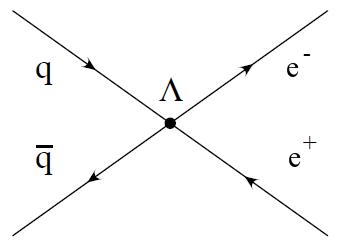
\includegraphics[scale=0.3]{images/fd2.png}
            %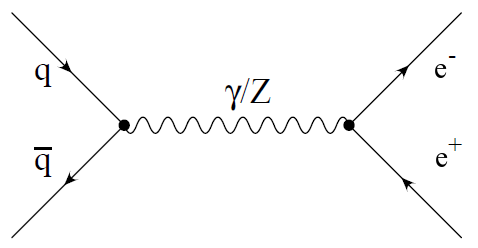
\includegraphics[scale=0.4]{images/fd1.png}
            \end{center}
            \caption{Feynman diagrams of a contact interaction (left) and the predominant background Drell-Yan production (right).}
            \label{fig:fd}
        \end{figure}

        Experimentally this interaction would be seen as a deviation from the Standard Model (SM) Drell-Yan (DY)($q\bar{q}~\rightarrow~\gamma/Z~\rightarrow~\ell^{+}\ell^{-}$) dilepton mass spectrum (seen in Fig. \ref{fig:fd}). 

        \begin{figure}[h]
            \begin{center}
            %\includegraphics[scale=0.3]{}
            \end{center}
            \caption{MC truth level comparison between DY spectrum without signal and with signal.}
            \label{fig:theoryInvMass}
        \end{figure}

        Without knowing the intermediate process one can write a Lagrangian describing the new Interaction; 

        \begin{equation}
            \mathcal{L} = \frac{g^{2}}{2\Lambda^{2}}
                [\eta_{LL} (\bar{\psi_{L}}\gamma_{\mu}\psi_{L}) (\bar{\psi_{L}}\gamma^{\mu}\psi_{L}) 
                + \eta_{RR} (\bar{\psi_{R}}\gamma_{\mu}\psi_{R}) (\bar{\psi_{R}}\gamma^{\mu}\psi_{R}) 
                + 2\eta_{LR} (\bar{\psi_{L}}\gamma_{\mu}\psi_{L}) (\bar{\psi_{R}}\gamma^{\mu}\psi_{R}) ]
        \end{equation}

        where $g$ is the coupling constant, $\Lambda$ is the energy scale of new physics and $\psi_{L}$ and $\psi_{R}$ are the left and right handed fermionic fields respectively. The sign of $\eta$ defines whether the new interaction interferes constructively ($\eta = -1$) or destructively ($\eta = +1$) with DY and is always unity. For previous analyses \cite{CDF, D0, ATLAS} a benchmark model of just the Left-Left (LL) component has been used and defined by $\eta_{LL} = \pm~1$ and $\eta_{RR} = \eta_{LR} = 0$. Here however an investigation of each of the three parameters is done individually. Both the LL and RR cases are expected to behave similarly however the LR case exhibits a different angular dependence than either of the other formalisms or the DY background. This difference is the primary reason for the inclusion of the angular part of this analysis found later. The discriminating variables used are therefore dilepton invariant mass and cosine of the decay angle $\theta^{*}$. The angle $\theta^{*}$ is defined in the Collins-Soper frame [\cite{PhysRevD.16.2219}] which is defined with the $x$-axis perpendicular to the incoming parton momentum frame and the $z$-axis bisecting the angle between the two incoming parton momenta. Since the incoming parton information is understandably unavailable the $z$-axis is taken as the direction of the incoming quark (as opposed to anti-quark) obtained from the boost in to the dilepton frame. The angle $\theta^{*}$ is then defined as the angle between this $z$-axis the momentum of the outgoing negatively charged lepton (or electron in this analysis).

        Figure \ref{fig:theoryAFB} shows the difference expected between the LR CI models and DY background from a truth Monte-Carlo study. The variables used are $A_{FB}$ and dilepton invariant mass where $A_{FB}$ is the forward-backwards asymmetry defined in relation to cos$\theta^{*}$ as;

        \begin{equation}
            A_{FB} = 
                \frac{N_{F} - N_{B}}{N_{F} + N_{B}}
            \label{eq:AFB}
        \end{equation}

        where $N_{F}$ and $N_{B}$ are number of events found with cos$\theta^{*}$ greater than 0 and less than 0 respectively.
        
        \begin{figure}[h]
            \begin{center}
            %\includegraphics[scale=0.3]{}
            \end{center}
            \caption{MC truth level comparison between the forward backwards asymmetry of DY and and of a CI LR signal.}
            \label{fig:theoryAFB}
        \end{figure}

        A differential cross section for this new interaction is given by

        \begin{equation}
            \frac{d\sigma}{dm_{\ell\ell}} = 
                \frac{d\sigma_{DY}}{dm_{\ell\ell}} 
                - \eta\frac{F_{I}}{\Lambda^{2}} 
                + \frac{F_{C}}{\Lambda^{4}},
            \label{eq:DiffCross}
        \end{equation}

        where $m_{\ell\ell}$ is the dilepton mass and $\Lambda$ is the scale of the new physics. In the case of quark/lepton compositness $\Lambda$ refers to the point at which fermions stop being bound as SM quarks and leptons. $F_{I}$ and $F_{C}$ define the interference DY-CI term and the pure CI term respectively. The scale of the interference and pure term vary with both the dilepton invariant mass as well as the scale of new physics $\Lambda$

        -- add angular difference




    \subsection{ADD Theory}
        %\addcontentsline{toc}{section}{ADD Theory}
        ADD is a theory used to solve the hierarchy problem via large extra spacial dimensions first described by Arkani-Hamed, Dimopoulos, and Dvali (ADD) \cite{ADD}. The ADD model predicts a graviton that propagates the extra dimensions and acquires Kaluza-Klein (KK) modes that show as a broad increase in the SM background. This is the reason the search for ADD is done in conjunction with CI.




\section{Past Searches}











